\documentclass[a4paper, 11pt]{article}
\usepackage{comment}
\usepackage{fullpage}
\usepackage{amsmath}
\usepackage{amssymb}
\usepackage{mathtools}
\usepackage{fontspec}
\usepackage{siunitx}
\defaultfontfeatures{Ligatures=TeX}
\usepackage{xfrac}
\usepackage{icomma}
\usepackage[section,below]{placeins}
\usepackage[labelfont=bf,font=small,width=0.9\textwidth]{caption}
\usepackage{subcaption}
\usepackage{graphicx}
\usepackage{grffile}
\usepackage{float}
\floatplacement{figure}{htbp}
\floatplacement{table}{htbp}
\usepackage{booktabs}
\usepackage{hyperref}
\begin{document}
\noindent
\centerline{\small{\textsc{Michigan State University}}} \\
\large{\textbf{CMSE/CSE 822 – Parallel Computing \hfill Fall 2019 \\
Homework 2}} \\
Alexander Harnisch \\
\noindent\makebox[\linewidth]{\rule{\textwidth}{0.4pt}}

\section*{1) Performance Modeling}
\subsection*{a)}
\label{sec:1a}
There is some missing information here and assumptions have to be made.
However, it's not important since it only effects the numbers to plug in and
get out, not the logic behind it.

The kernel performs 6 floating point operations (FLOP) in each iteration.
Assuming no caching we have seven floating point number reading and one writing
operation for each loop iterations. However, we can assume that the same
variables are kept in the registers in each loop iterations, or at least in
fast memory. Which means the entire $y$ and $z$ arrays both only have to be
loaded once. Assuming single precision with $\SI{4}{byte}$ per float that
translates to $\SI{12}{byte}$ of memory access and an arithmetic intensity $I$
of
\begin{equation}
  I = \frac{\SI{6}{FLOP}}{\SI{12}{byte}} = \frac{1}{2}\,\frac{\textup{FLOP}}{\textup{byte}}\,.
\end{equation}

\subsection*{b)}
In a simple roofline model for some $I$ the critical peak performance
$\pi_\textup{crit}$ is given by $\beta I$, where $\beta$ is the peak memory
bandwidth. So for $I = 0.5\,\frac{\textup{FLOP}}{\textup{byte}}$ from
\hyperref[sec:1a]{a)} we get:
\begin{equation}
  \pi_\textup{crit} = 30\,\frac{\textup{GB}}{\textup{s}}\cdot \frac{1}{2}\,\frac{\textup{FLOP}}{\textup{byte}} = 15\,\frac{\textup{GFLOP}}{\textup{s}}\,.
\end{equation}
So in case the processor's peak performance is greater than
$\SI{15}{GFLOP\per\second}$ the kernel is compute bound, otherwise
memory bound.

\newpage
\subsection*{c)}
A simple roofline model plot is given by Figure~\ref{fig:roofline}. The
performance for an arithmetic intensity of $I = \SI{0.5}{FLOP\per byte}$ is
$\SI{15}{GFLOP\per\second}$.
\begin{figure}
  \centering
  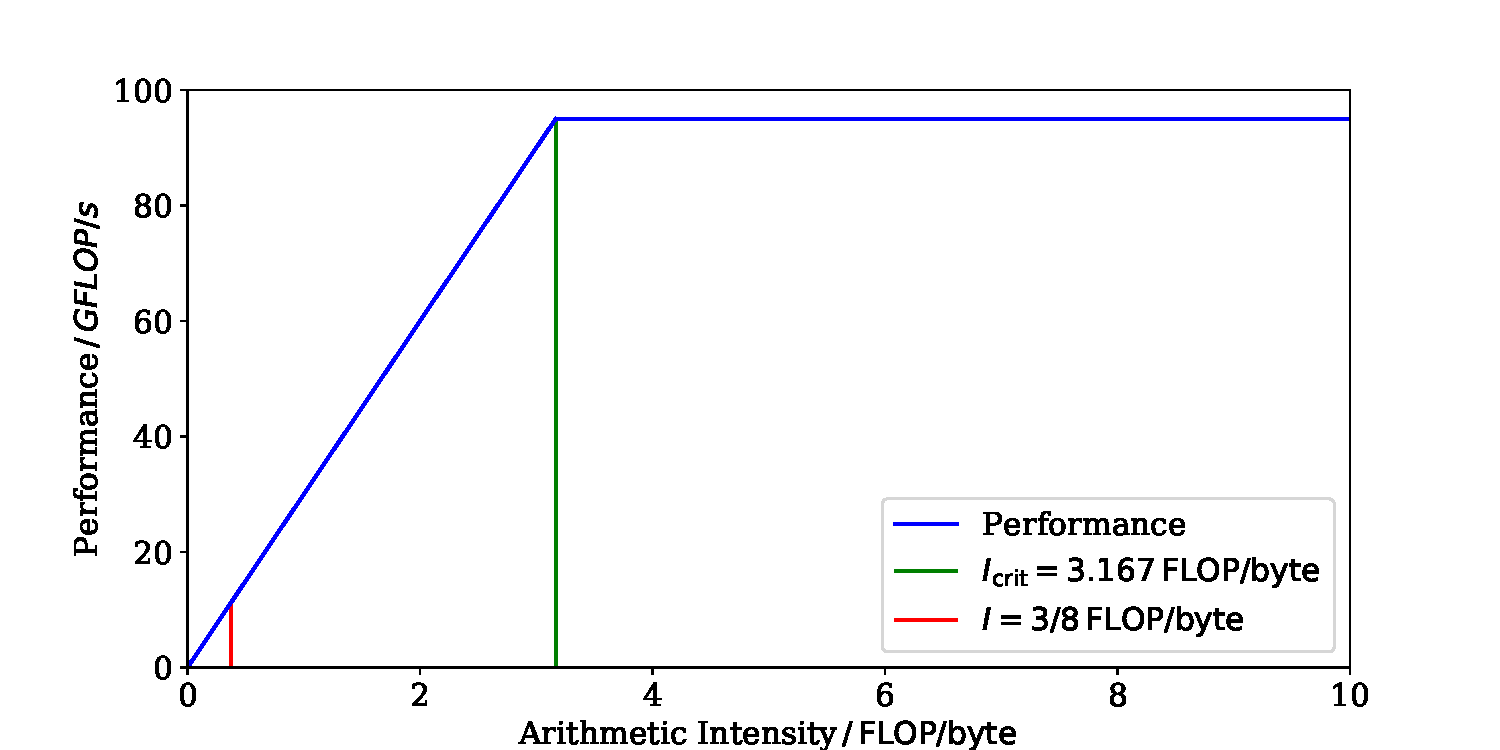
\includegraphics[width=\textwidth]{../plot/roofline.pdf}
  \caption{Simple roofline model.}
  \label{fig:roofline}
\end{figure}

\section*{2) Cache optimization: Matrix Vector Multiplication}

\subsection*{a) Implementation}
See code in repository.

\subsection*{b) and c) Performance Analysis and Cache Performance Measurement}
For all of the testing in this subsection, scripts for fully automated job
submission and data collection have been written in \textsc{Bash} and
\textsc{Python}. Using this system, 1968 different sets of parameters ($N$,
$M$ and $B$) were tested. For each run the relative speedup as well as cache
misses for L1, L2 and L3 were collected as variables of interest. All of the
results are summarized in the following plots. The raw data can be found in the
file \textit{data.txt} in my repository, outside of the submission directory.

Figure~\ref{fig:all_runs} shows the speedup for all tested matrices in
dependence of the blocking factor $B$. Each data point is the average speedup
for all matrices with the corresponding $B$ value.
\begin{figure}
  \centering
  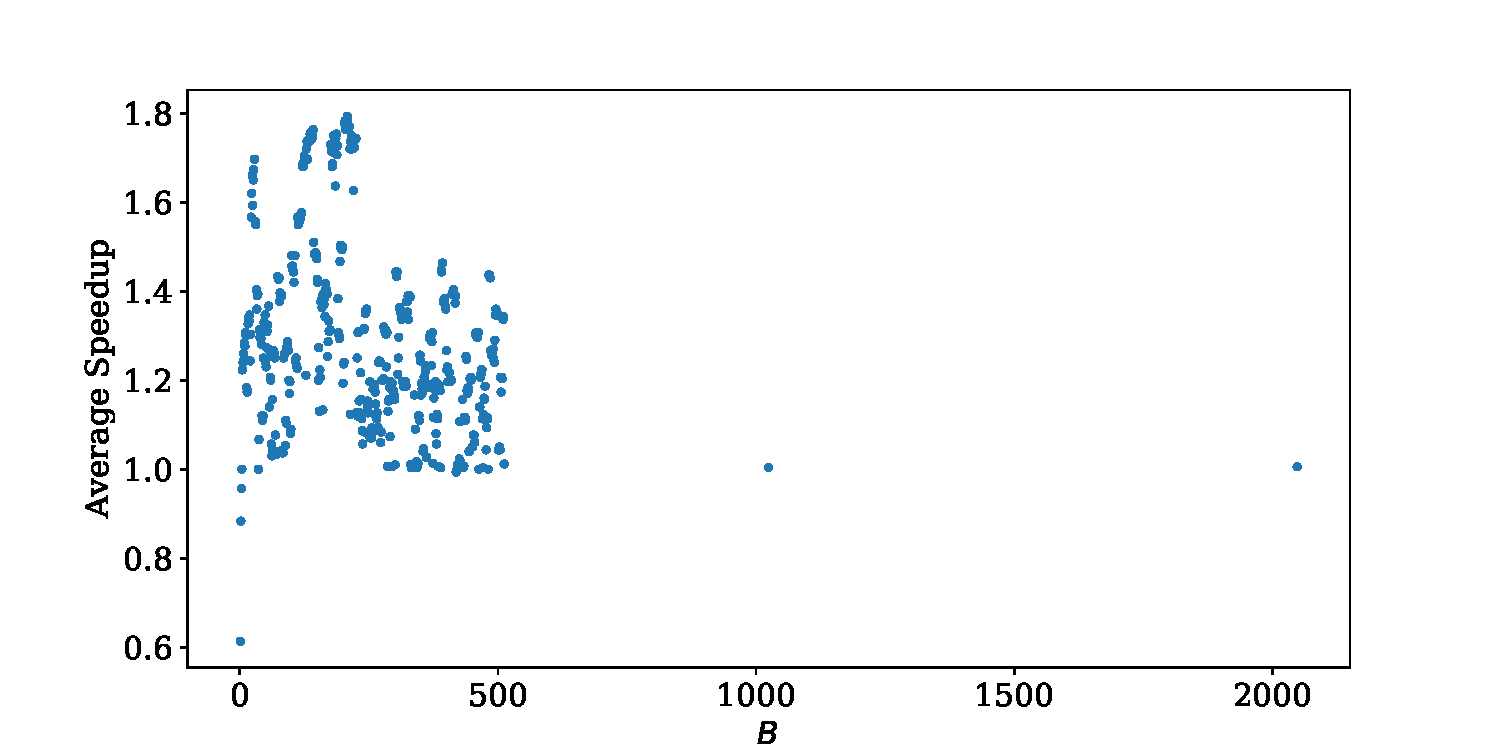
\includegraphics[width=\textwidth]{../plot/speedup_for_all_bs.pdf}
  \caption{Average speedup for all tested matrices in dependence of the blocking factor $B$.}
  \label{fig:all_runs}
\end{figure}

\begin{figure}
  \centering
  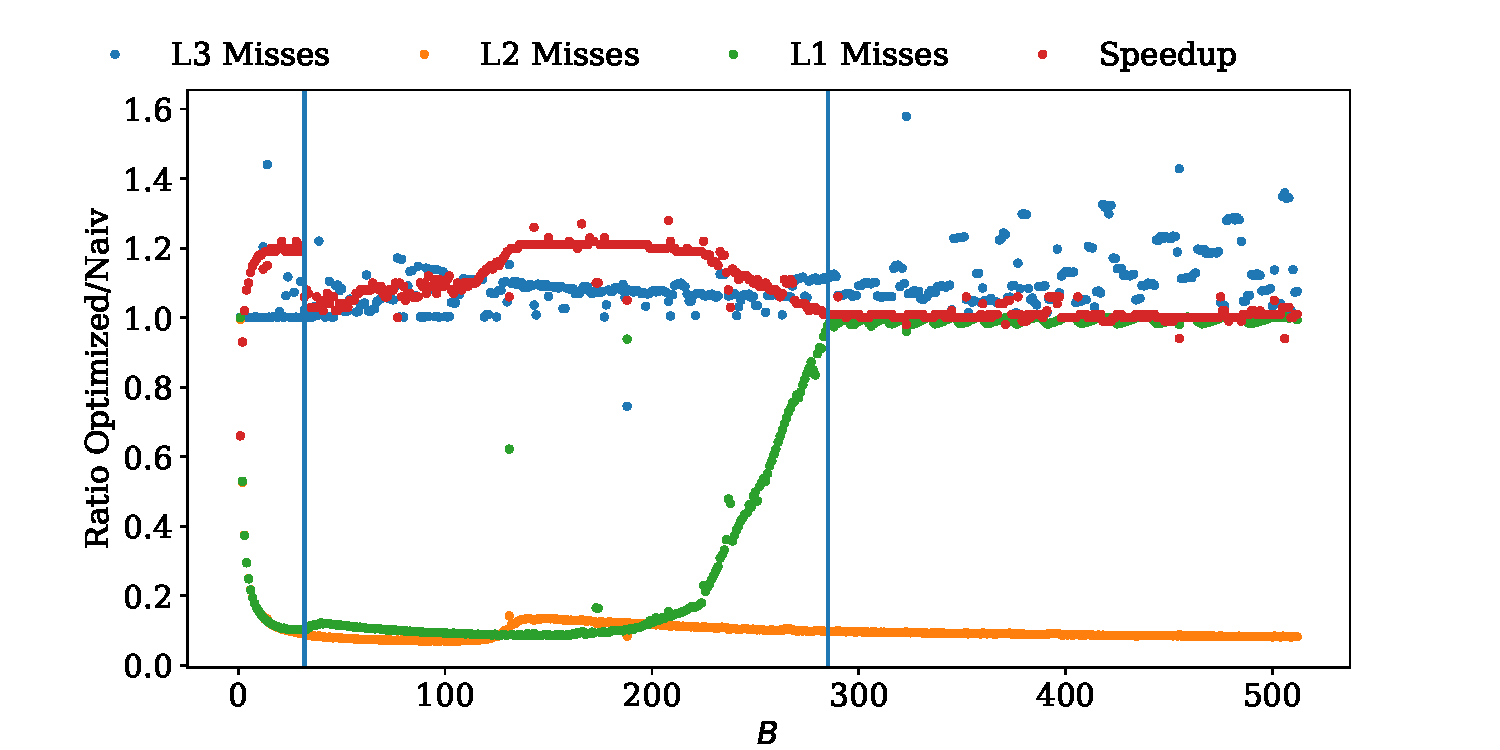
\includegraphics[width=\textwidth]{../plot/square_against_B.pdf}
  \caption{Results for a fixed matrix size of $N = M = 10000$ for different
  blocking factors $B$. For reference, the plot includes two blue vertical lines
  at $B=32$ and $B=285$.}
  \label{fig:square_against_B}
\end{figure}

\begin{figure}
  \centering
  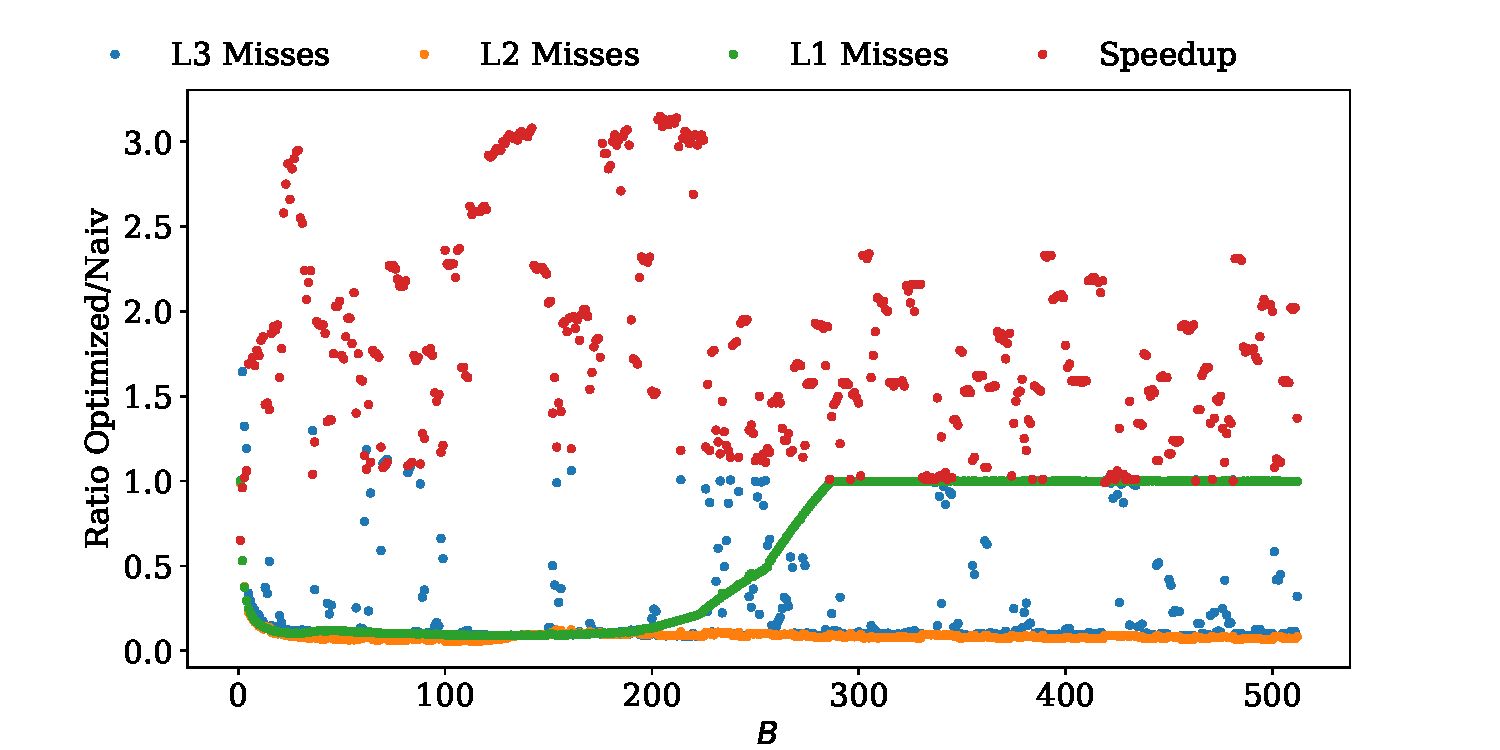
\includegraphics[width=\textwidth]{../plot/narrow_against_B.pdf}
  \caption{Results for a narrow matrix with $N=100000$ and $M=200$ for different blocking factors $B$.}
  \label{fig:narrow_against_B}
\end{figure}

\begin{figure}
  \centering
  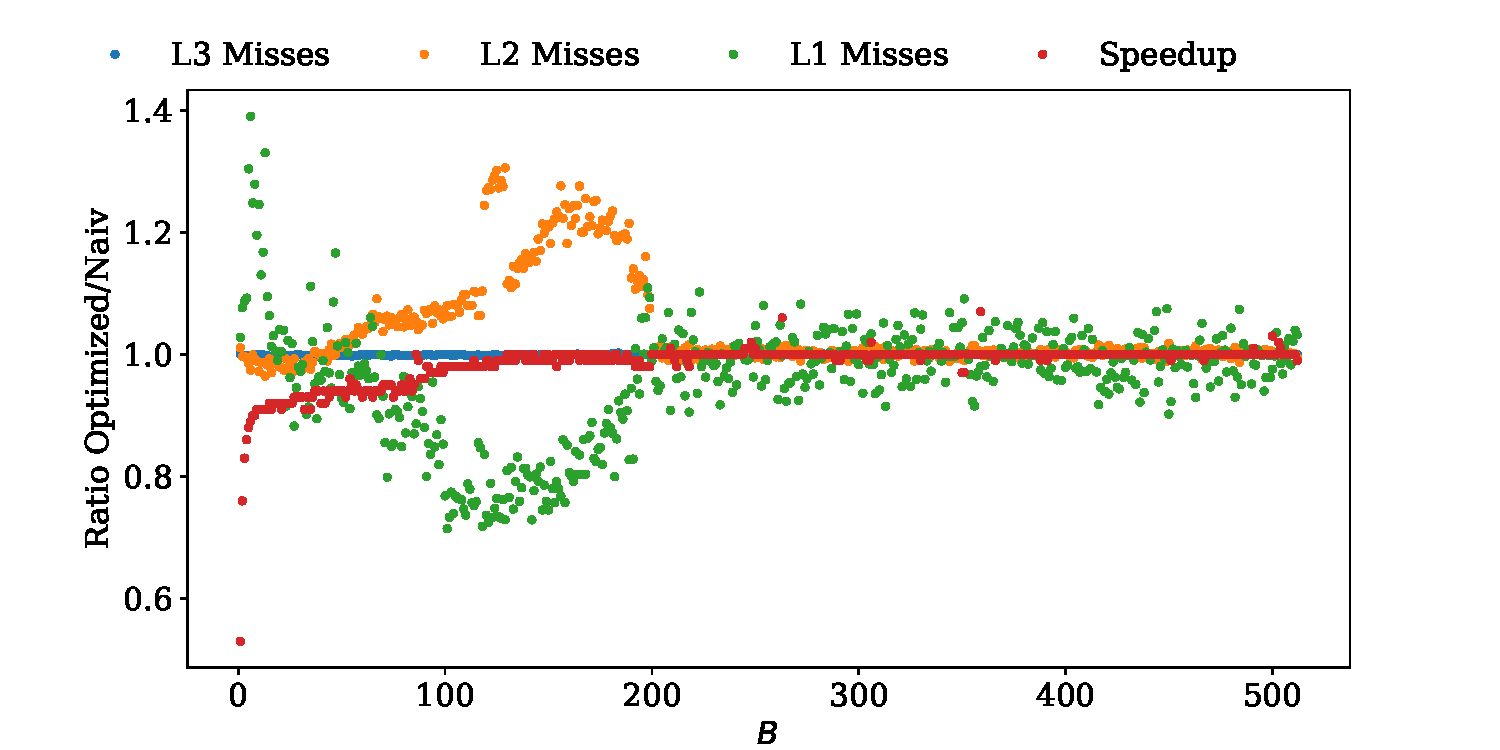
\includegraphics[width=\textwidth]{../plot/wide_against_B.pdf}
  \caption{Results for a wide matrix with $M=100000$ and $N=200$ for different blocking factors $B$.}
  \label{fig:narrow_against_B}
\end{figure}

\begin{figure}
  \centering
  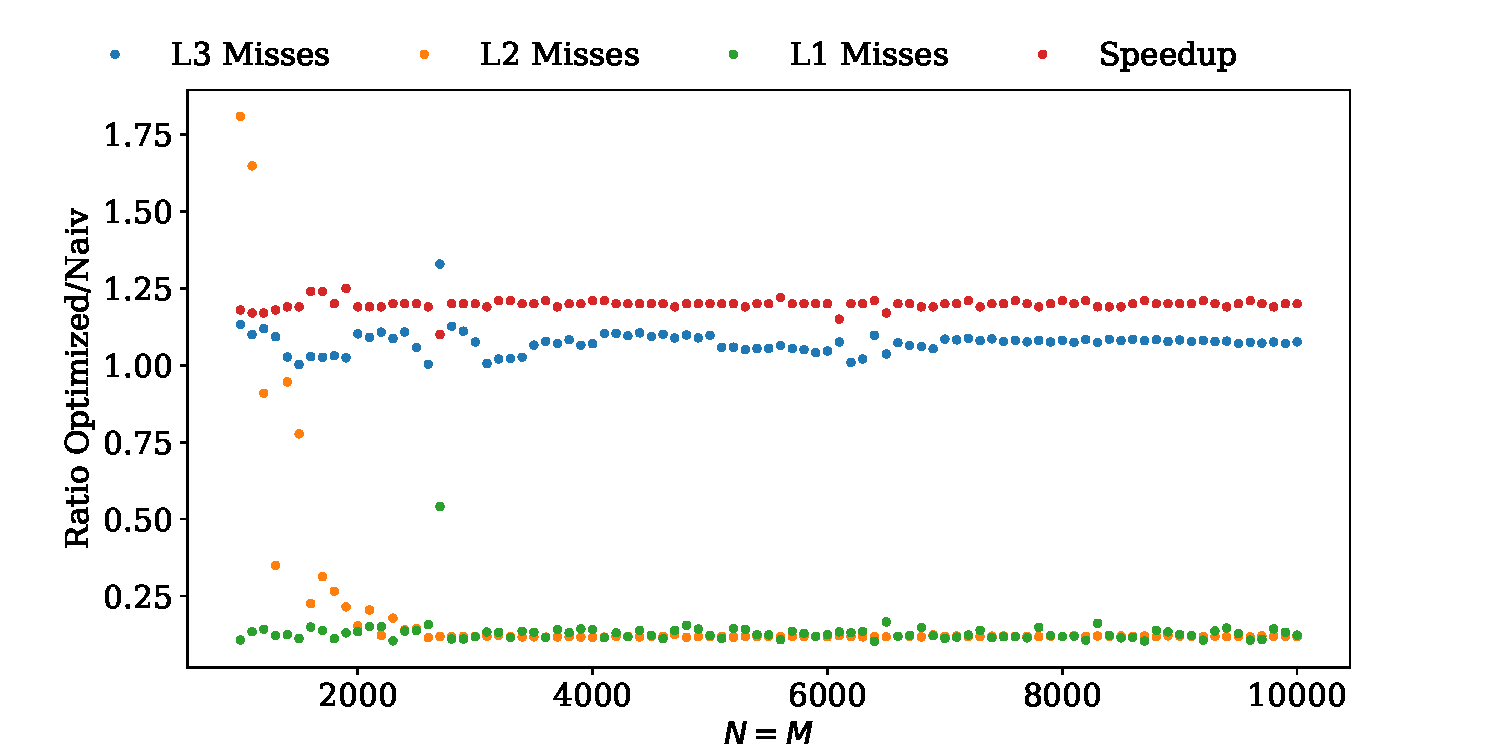
\includegraphics[width=\textwidth]{../plot/fixed_B_different_squares.pdf}
  \caption{Results for a fixed blocking factor of $B=200$ for different square matrices ($N = m$).}
  \label{fig:fixed_B_different_squares}
\end{figure}

\begin{figure}
  \centering
  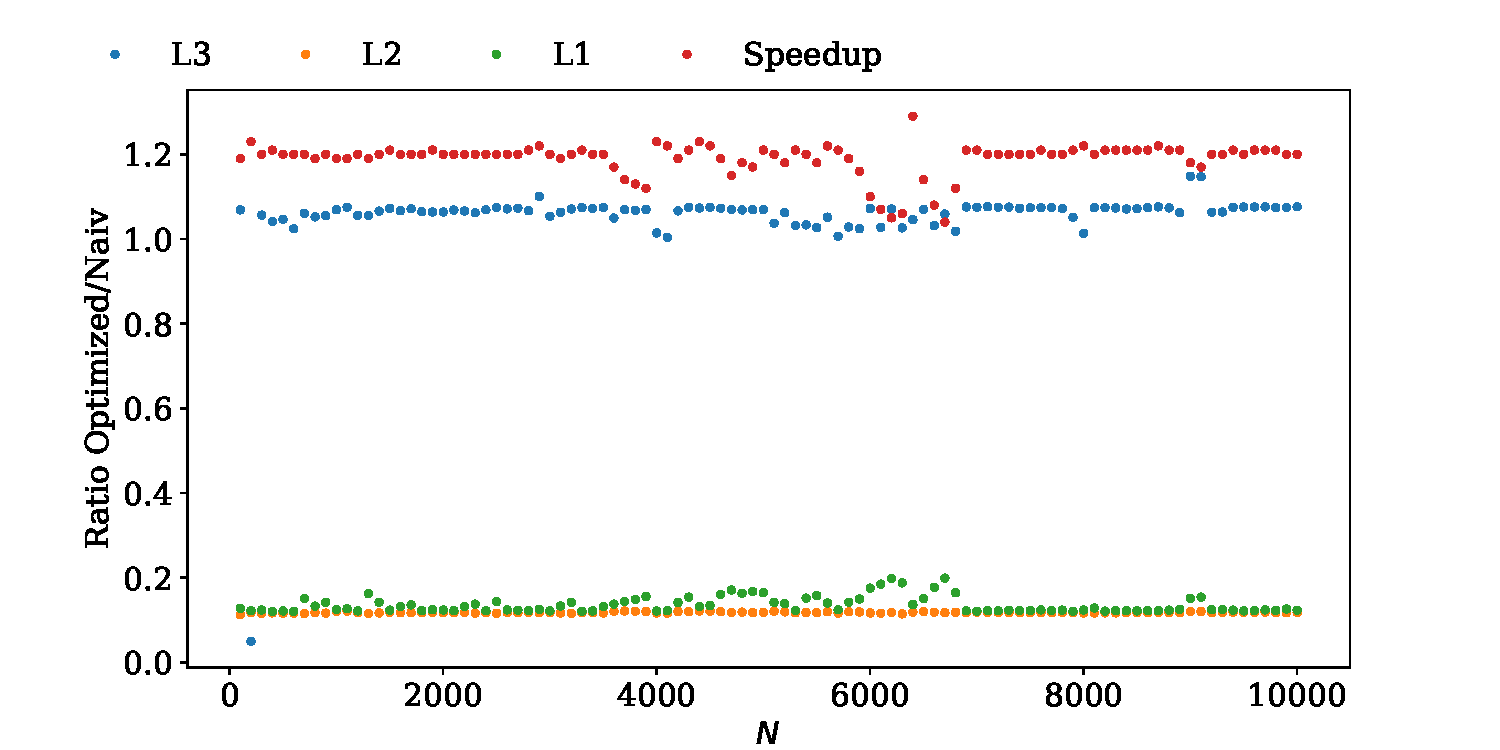
\includegraphics[width=\textwidth]{../plot/fixed_B_M_different_N.pdf}
  \caption{Results for a fixed blocking factor of $B=200$ and fixed $M=10000$
  for different $N$.}
  \label{fig:fixed_B_M_different_N}
\end{figure}

\begin{figure}
  \centering
  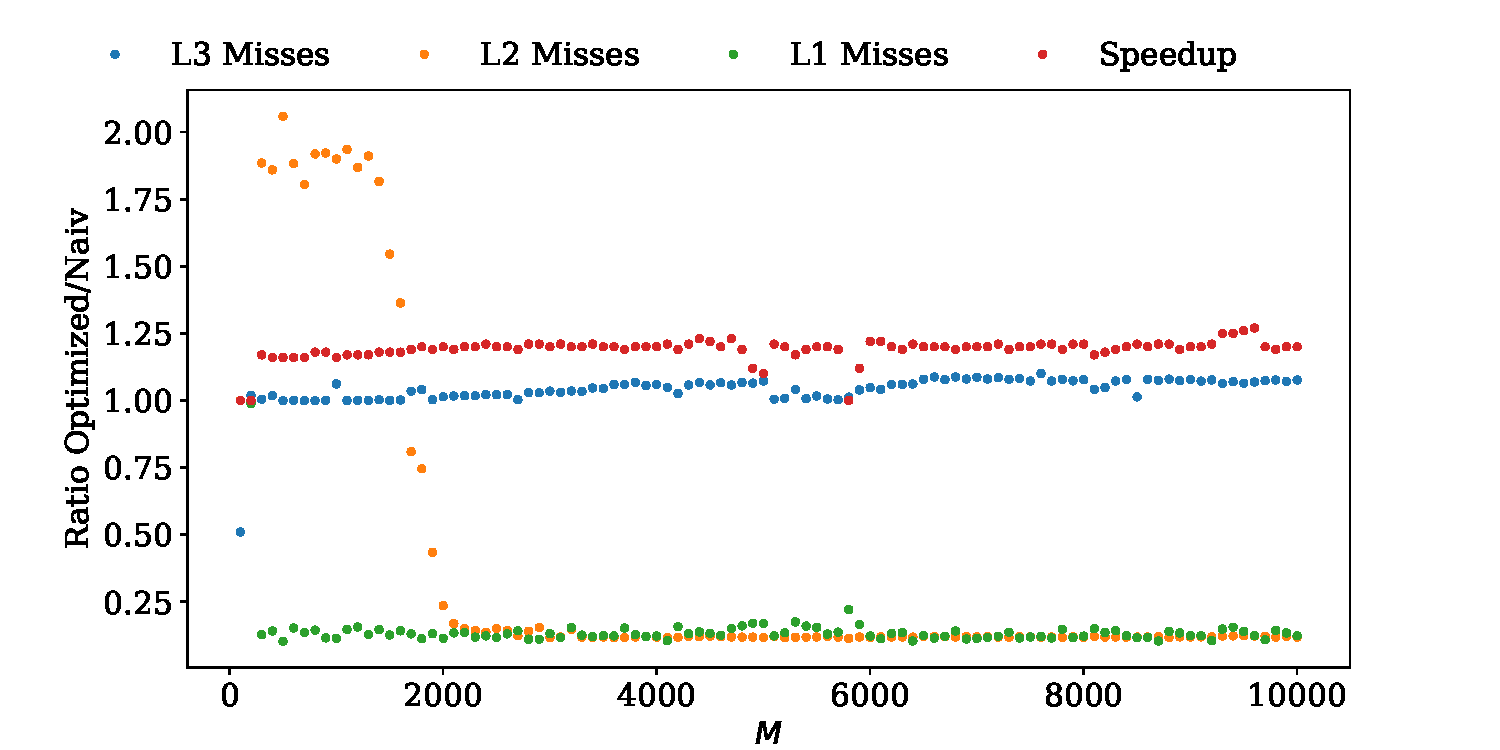
\includegraphics[width=\textwidth]{../plot/fixed_B_N_different_M.pdf}
  \caption{Results for a fixed blocking factor of $B=200$ and fixed $N=10000$
  for different $M$.}
  \label{fig:fixed_B_N_different_M}
\end{figure}

\subsection*{d) Inference about the Memory Hierarchy}
\end{document}
